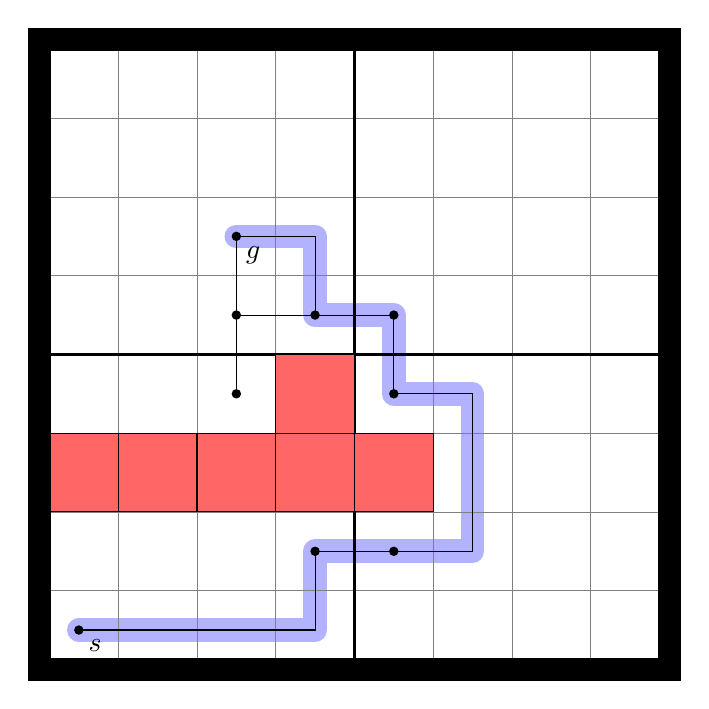
\begin{tikzpicture}
[
	bline/.style={line width=0.3cm,cap=round,join=round, color=blue!30},
	obst/.style={fill=red!60},
	myNodeLine/.style={thin,color=black!100}
]

\def\square{rectangle +(1,1)}
\def\entranceNode{circle (0.06cm)}
% Draw path
% Final path
\draw[bline] (0.5,0.5)--(3.5,0.5)--(3.5,1.5)--(5.5, 1.5)--(5.5, 3.5)--(4.5, 3.5)--(4.5, 4.5)--(3.5,4.5)--(3.5, 5.5)--(2.5,5.5);

% Draw grid 	
\draw[help lines] (0,0) grid (8,8);

% Create cluster lines
\draw[thick] (0,4)--(8,4);
\draw[thick] (4,0)--(4,8);

% Draw obstacle
\draw[obst] (2, 2) \square (3, 2) \square  (3, 3) \square  (4, 2) \square  (1, 2) \square (0, 2) \square;

% Draw border
\draw[line width=0.3cm] (0,0) rectangle +(8,8);

% Draw nodes
\draw[below right] (0.5, 0.5) node(s){$s$};
\draw[below right] (2.5, 5.5) node(t){$g$};
\fill (0.5,0.5) circle (0.06cm) (2.5,5.5) circle (0.06cm);

% Draw lines between nodes
\draw[myNodeLine](2.5, 3.5)--(2.5, 4.5) 
										(3.5, 4.5)--(4.5, 4.5) 
										(3.5, 1.5)--(4.5, 1.5);
										(4.5, 3.5)--(4.5, 4.5);

% Draw intra cluster edges
\draw[myNodeLine](4.5, 1.5)--(5.5, 1.5)--(5.5, 3.5)--(4.5, 3.5)--(4.5, 4.5)--(2.5,4.5);

% Draw connections to start and goal
\draw[myNodeLine](0.5, 0.5)--(3.5, 0.5)--(3.5, 1.5) (2.5, 5.5)--(2.5, 4.5) (2.5,5.5)--(3.5, 5.5)--(3.5, 4.5);

% Create entrance nodes
\fill (4.5,1.5) \entranceNode (3.5, 1.5) \entranceNode;
\fill (3.5, 4.5) \entranceNode (4.5, 3.5) \entranceNode;
\fill (4.5, 4.5) \entranceNode;
\fill (2.5, 4.5) \entranceNode (2.5, 3.5) \entranceNode;

\end{tikzpicture}